\chapter{Rozproszone serwery WWW}
\label{r03}
Rozdział ten przybliży architekturę najczęściej wykorzystywaną w komunikacji tak pomiędzy programami jak i
urządzeniami sieciowymi: architekturę klient--serwer. Następnie zostanie przedstawiona budowa i działanie serwera
WWW oraz współpracującego z nim klienta -- przeglądarki. Kolejnym punktem tego rozdziału będzie klasyfikacja
serwerów WWW ze względu na wielkość obsługiwanego ruchu jak i na charakterystykę budowy i wymagania oraz
związane z tym definicje. W ostatnim punkcie tego rozdziału będzie przedstawiony sposób testowania serwerów webowych.

\section{Wprowadzenie}
Częstość i wydajność dostarczania usług WWW, przy stale zwiększającej się ich popularności, 
stanowi nie lada problem dla tradycyjnych rozwiązań klient--serwer. Zwiększenie dostępności
serwisów można osiagnąć modyfikując poszczególne elementy na drodze od klienta do serwera 
i/lub dodając nowe. Na rys. \ref{www} przedstawiono część elementów, które wpływają na wydajność 
sieci Web.
\begin{figure}[h]
\centering
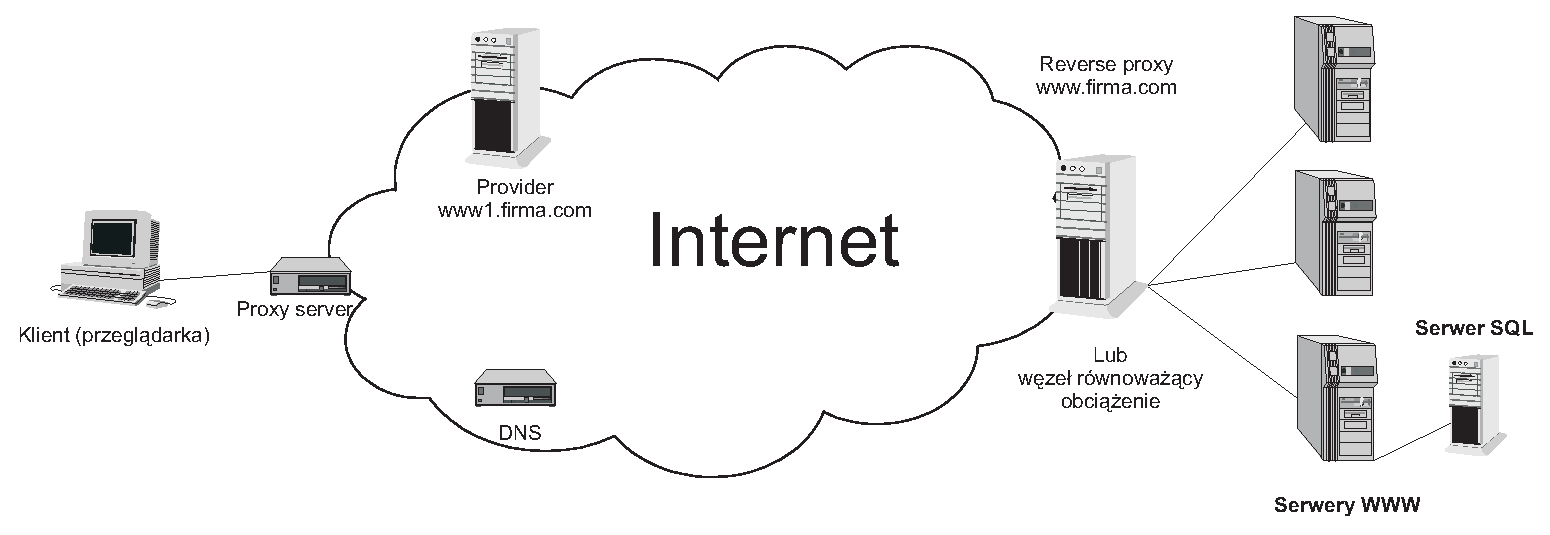
\includegraphics[width=\textwidth]{./rysunki/www.eps}
\caption{Przykładowe elementy stanowiące o wydajności WWW}
\label{www}
\end{figure}

Najprostszymi są \emph{cache} przeglądarki lub proxy serwer zainstalowany
po stronie klienta. Takie rozwiązanie ma wiele zalet: prostota instalacji i konfiguracji, a przy
odpowiednich dokumentach (statyczny HTML) efektywność takiego rozwiązania jest bardzo duża. 
Wadą tych rozwiązań jest głównie słaba wydajność przy dokumentach generowanych dynamicznie
(a takich obecnie zdarza się coraz więcej). Podobne rozwiązanie można zastosować po stronie 
serwera WWW, tzn. proxy, które keszuje strony po stronie serwera(ów) -- nazywa się ono 
\emph{reverse proxy}. 

Można także skorzystać z usług różnych dostawców (\emph{providerów})
i przenieść część witryny WWW na ich komputery. Efektem będzie zwiększenie dostępności 
(oraz wydajności) witryny, jednakże za cenę mniejszego bezpieczeństwa i zmniejszenia 
funkcjonalności sajtu.

Można zwiększać wydajność w najprostszy sposób --
poprzez dodawanie kolejnych procesorów, pamięci, dysków czy też urządzeń sieciowych. Jest to 
możliwe tylko w bardzo ograniczonym zakresie. 

Wydaje się, że najciekawszym rozwiązaniem
jest wielokomputerowy serwer WWW. Zaletą wykorzystania wielokomputerowego serwera WWW
jest praktycznie nieograniczona skalowalność i wysoka dostepność, wadą natomiast -- 
propagowanie ruchu na poszególne jego składowe (nody). Zarządzanie ruchem można realizować na
szereg sposobów: poprzez \emph{reverse proxy}, na poziomie serwera DNS, poprzez osobny węzeł
równoważący obciążenie, modyfikując usługi po stronie klienta (opisane dalej applety Java), lub
serwera (metody te zostały opisane w rozdziale \ref{r03}). Wraz z architekturą takiego systemu zarządzającego serwerem WWW
należy zaprojektować algorytmy umożliwiające rozpraszanie ruchu sieciowego (Rozdział \ref{r04}).
Część wyżej wymienionych rozwiązań może być tak iprogramowa jak i sprzętowa.

\section{Model klient--serwer}

\hspace{0.63cm}Model współpracy klient--serwer to taki model, w którym jeden program czeka pasywnie na żądanie komunikacji
wysyłane przez inne programy. Określenia klient i serwer odpowiadają dwóm programom zaangażowanym w wymianę informacji.
Program inicjujący połączenie nazywany jest klientem, a program biernie czekający na żądanie połączenia -- serwerem. Charakterystyka modelu \cite{siecikomputerowe}:

\begin{description}
\item[Oprogramowanie klienta]\
\begin{itemize}
\item dowolny program użytkowy, który staje się klientem tymczasowo (w trakcie komunikacji), ale wykonuje również obliczenia
lokalnie;
\item jest wywoływane bezpośrednio przez użytkownika na czas obejmujący jedną sesję;
\item działa lokalnie na urządzeniu osobistym użytkownika;
\item aktywnie inicjuje połączenie z serwerem;
\item w razie potrzeby może komunikować się z wieloma serwerami, jednak naraz aktywnie komunikuje się tylko z jednym;
\item nie wymaga specjalnego sprzętu, ani spesjalizowanego systemu operacyjnego.
\end{itemize}
\item[Oprogramowanie serwera]\
\begin{itemize}
\item jest specjalizowanym programem, którego zadaniem jest świadczenie konkretnej usługi -- może obsługiwać naraz wielu
klientów;
\item jest programem uruchamianym podczas startu systemu i działa przez wiele kolejnych sesji;
\item działa na publicznie dostępnym komputerze;
\item czeka na zgłaszanie się programów klienckich;
\item pełni konkretną usługę, ale połączenia przyjmuje od dowolnych odległych klientów;
\item wymaga specjalnego sprzętu i wyrafinowanego systemu operacyjnego.
\end{itemize}
\end{description}

\section{Architektura WWW}

\subsection{Serwer WWW}

\hspace{0.63cm}Najprościej opisać serwer WWW jako program wykonujący w pętli prostą operację: czekanie na otwarcie połączenia przez klienta
(przeglądarkę) czyli na wysyłanie przez niego żądania dostępu do określonej strony. W odpowiedzi serwer wysyła żądany dokument 
(lub komunikat o błędzie w razie jego braku) albo przekazuje połączenie do realizacji modułowi (np. odpowiedzialnemu za obsługę
CGI) lub innemu serwerowi (np.: baz danych). następnie serwer zamyka połączenie i czeka na następne. 

\subsection{Klient WWW -- przeglądarka}

\hspace{0.63cm}Przeglądarki WWW mają bardziej złożoną budowę niż serwery WWW. Obsługuje ona większość zagadnień związanych
z dostępem do dokumentów i ich pokazywaniem użytkownikowi. W związku z tym składa się ona z szeregu dużych modułów, które
ze sobą współdziałają \cite{siecikomputerowe}.

Koncepcyjnie przeglądarka składa się z zestawu klientów, interpreterów i modułu, który tym wszystkim zarządza. Moduł
centralny -- zarządzający jest odpowiedzialny za interpretację danych z klawiatury i myszki oraz za wywołania pozostałych
modułów w celu wykonania operacji żądanych przez użytkownika.

\begin{figure}[h]
\centering
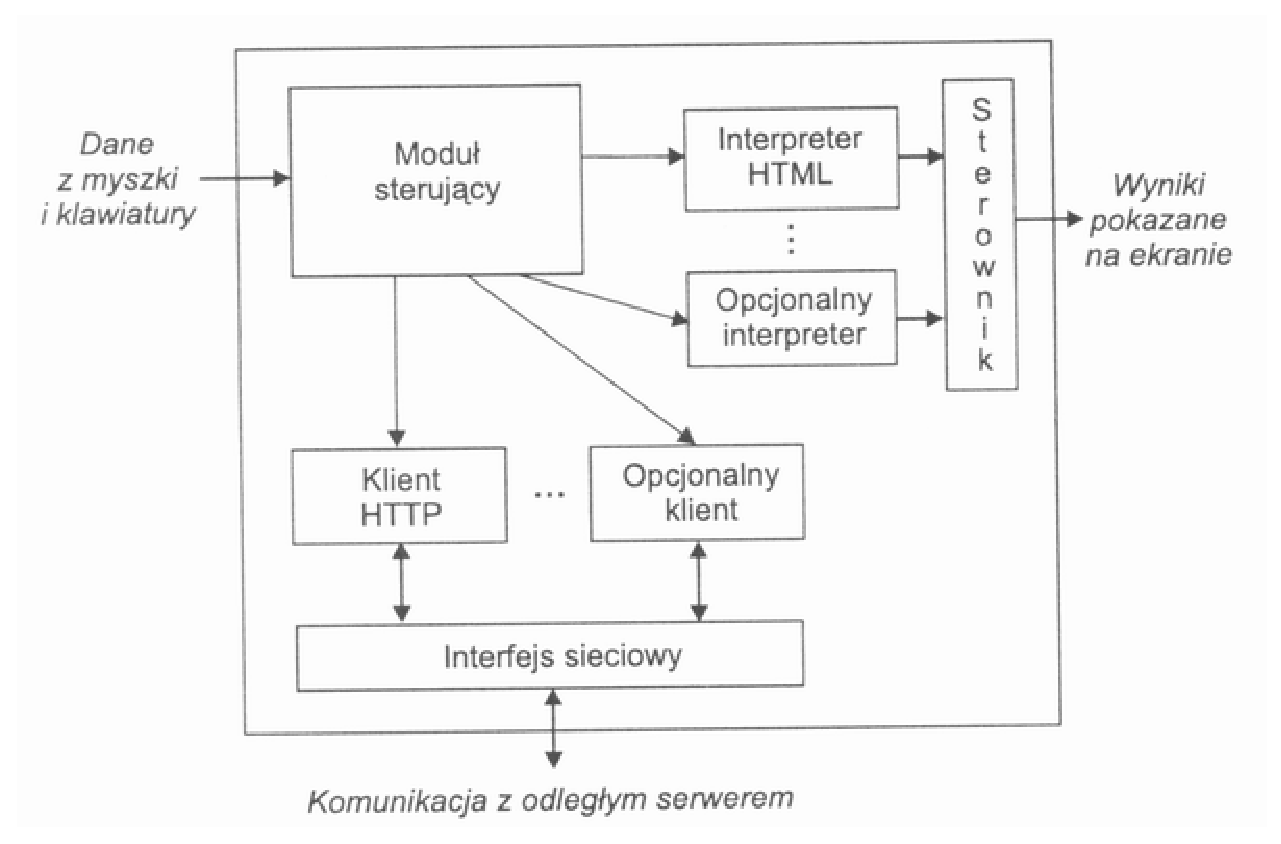
\includegraphics[width=4in]{./rysunki/przeg.eps}
\caption{Główne składniki przeglądarki WWW}
\label{przeglądarka}
\end{figure}

Każda przeglądarka musi zawierać interpreter języka HTML, żeby w ogóle mogła interpretować dokumenty WWW. Inne interpretery
są opcjonalne, jednakże powoli stają się również niezbędne -- takie jak interpreter Javy, czy XML. Dane dla interpretera
HTML stanowi dokument o zawartości zgodnej ze składnią tego języka; wynikiem jego działania jest sformatowana postać
dokumentu przez zamianę znaczników formatujących na polecenia sterujące sprzętem wyświetlającym informacje.

Jedną z najważniejszych funkcji interpretera HTML jest obsługa fragmentów dokumentu wybieralnych przez użytkownika.
Interpreter musi przechowywać informacje o związku między pozycjami na ekranie, a odsyłaczami w dokumencie HTML. Gdy
użytkownik wskazuje za pomocą myszki pozycję w dokumencie, interpreter HTML na podstawie bieżącej pozycji kursora i
zapamiętanych informacji ustala, który odsyłacz wskazał użytkownik.

\subsection{Podział serwerów WWW}

\hspace{0.63cm}Serwery WWW można scharakteryzować głównie poprzez wielkość (ilość realizacji żądań) \cite{wybraneelementy}:
\begin{description}
\item[małe] -- uruchamiane na stacjach roboczych, zdolne do obsłużenia do 5000 zapytań dziennie, np.: prezentujące dane jakiejś
niewielkiej firmy;
\item[średnie] -- uruchamiane na dużych serwerach posiadających zabezpieczenia na poziomie urządzeń wewnętrznych. Obsługują
kilkadziesiąt tysięcy żądań dziennie. Prezentują dane (tysiące stron) średniej firmy;
\item[duże] -- uruchamiane na serwerach o dużej mocy obliczeniowej (zwykle kilku) posiadających techniki zabezpieczenia
danych i pracy serwerów. Są w stanie obsłużyć kilkaset tysięcy zapytań dziennie (prezentują kilkaset tysięcy stron);
\item[globalne] -- są w stanie obsłużyć milion żądań klienckich dziennie, prawie zawsze zbudowane z wielu dużych serwerów, 
posiadające kilka kopii dokumentu. Są wstanie udostępniać ogromne ilości danych , również multimedialnych.
\end{description}
W zależności od zawartości witryn definiuje się trzy klasy obciążalności serwerów WWW \cite{ScalableWebClusters}. Mamy zatem 
witryny typu:
\begin{description}
\item[web publishing] -- witryny zawierające statyczne i w niewiekiej ilości dynamiczne dokumenty. Dokumenty statyczne są 
składowane na dyskach serwera webowego i nie podlegają modyfikacjom przez relatywnie długi czas i zawsze są przechowywane w 
pamięci podręcznej. Pamięć podręczna każdego nodu klastra jest zwykle ustawiona na 15\% całkowitego drzewa dokumentów witryny.
Strony w niewielkim stopniu dynamiczne są przechowywane w pamięci podręcznej (cache) z pradopodobieństwem 0,3.
\item[web transaction (light)] -- są to witryny zawierające około 60\% dokumentów statycznych i około 40\% stworzonych 
dynamicznie dokumentów. Zapytania bazodanowe do serwerów \emph{back--endowych} wymagają intensywanego korzystania z dysków i 
stąd rezultaty zapytań nie są przechowywane w keszu.
\item[web transaction (heavy)] -- witryny zawierające 30\% statycznych dokumentów, 30\% niewiele zdynamizowanych dokumentów
oraz różne kombinacje (dla pozostałych 40\%) dokumentów, zwykle zawierających elementy wymagające sporych mocy obliczeniowych 
CPU i/lub dysku.
\end{description}

\section{Charakterystyka wydajności serwera WWW}

Podstawową miarą obciążenia serwera WWW jest ilość żądań HTTP, które docierają do niego w ciągu sekundy. 
Za miarę wydajności serwera można przyjąć widziany od strony klienta czas odpowiedzi na żądanie lub czas 
ukończenia transferu dokumentu, który zależny jest jednak od przepustowości połączenia klienta z Internetem. 
Przeprowadzone w USA symulacje z użyciem prostego modelu serwera WWW, który oparto o teorię kolejek i założenie, 
że istotne są tylko żądania typu GET, są podstawą do przedstawienia poniższych charakterystyk.
Typowo czas odpowiedzi na żądanie rośnie wraz ze wzrostem liczby żądań na sekundę. Wzrost ten jest 
początkowo bardzo powolny, niemal niezauważalny aż do momentu, w którym ilość równocześnie otwartych połączeń 
TCP przekracza możliwości obsługi ich przez serwer. Przedstawia rysunek \ref{zapytania}[26].
\begin{figure}[h]
\centering
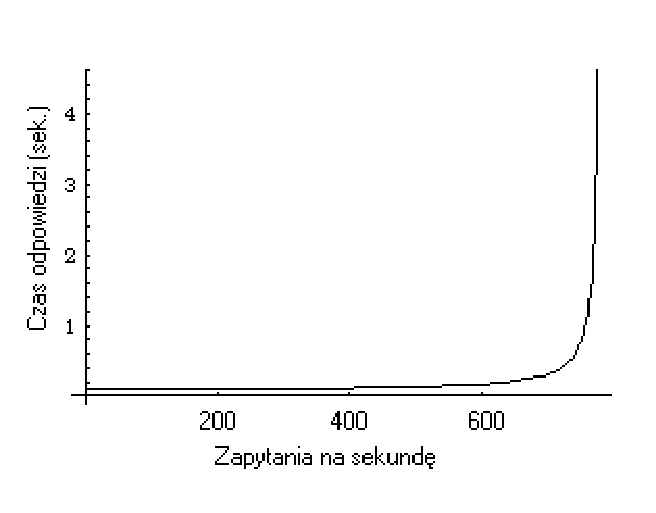
\includegraphics[width=3in]{./rysunki/zapytania.eps}
\caption{Czas odpowiedzi a ilość zapytań na sekundę.}
\label{zapytania}
\end{figure}

Obciążenie przy którym serwer załamuje się zależy oczywiście od 
sprzętowych własności serwera i zastosowanego oprogramowania. Oprócz cech samego serwera najistotniejsze dla 
czasu odpowiedzi są przepustowość połączenia z Internetem oraz średni rozmiar plików wysyłanych przez serwer. 
Średni rozmiar pliku zależy w głównej mierze od rodzaju informacji publikowanych na serwerze (będzie on np. duży 
na serwerze oferującym wiele plików video). Pożądane jest jednak ,,oszczędne'' projektowanie stron WWW, gdyż 
wzrost średniego rozmiaru pliku powoduje szybki spadek ilości zapytań na sekundę możliwych do obsłużenia. 
Opisane zachowanie 
serwera powodujące załamanie się jego wydajności po przekroczeniu maksymalnej liczby zapytań na sekundę jest 
typowe dla implementacji nie posiadających ograniczenia na maksymalną liczbę jednoczesnych połączeń TCP. Dotyczy 
to większości systemów UNIX--owych, w których procesy serwerów WWW wykonują standardową akcję fork--and--exec dla 
każdego nowego żądania HTTP. Prostym rozwiązaniem tego problemu wydaje się wprowadzenie ograniczenia na liczbę 
połączeń TCP. Wymagałoby to jednak zmian w protokole HTTP (np. wprowadzenie odpowiedzi typu ,,serwer zajęty --
spróbuj później'') oraz odpowiednich zmian w przeglądarkach.

Powyższe rozważania dotyczą wydajności serwera widzianej od strony klienta. W przypadku laboratoryjnych 
badań wydajności łatwiej niż czas odpowiedzi można zmierzyć ilość zapytań na sekundę obsługiwaną przez serwer. 
Jest to miara wydajności bezpośrednio korespondująca z czasem odpowiedzi serwera (im więcej zapytań serwer może 
obsłużyć, tym mniejszy jest jego czas reakcji) i wolna od wpływu takich czynników jak wydajność przyłącza po 
stronie klienta.
Ciągły wzrost liczby użytkowników Internetu stawia coraz większe wymagania co do wydajności serwerów WWW. Do tego faktu dochodzi jeszcze jeden - charakterystyka ruchu WWW - oprócz serwowania stron statycznych, dochodzą dynamiczne i obsługa połączeń szyfrowanych. 
W jaki sposób zmienia się wtedy wykorzystanie poszczególnych elementów widać na rys.\ref{charakterystyka}
\begin{figure}[h]
\centering
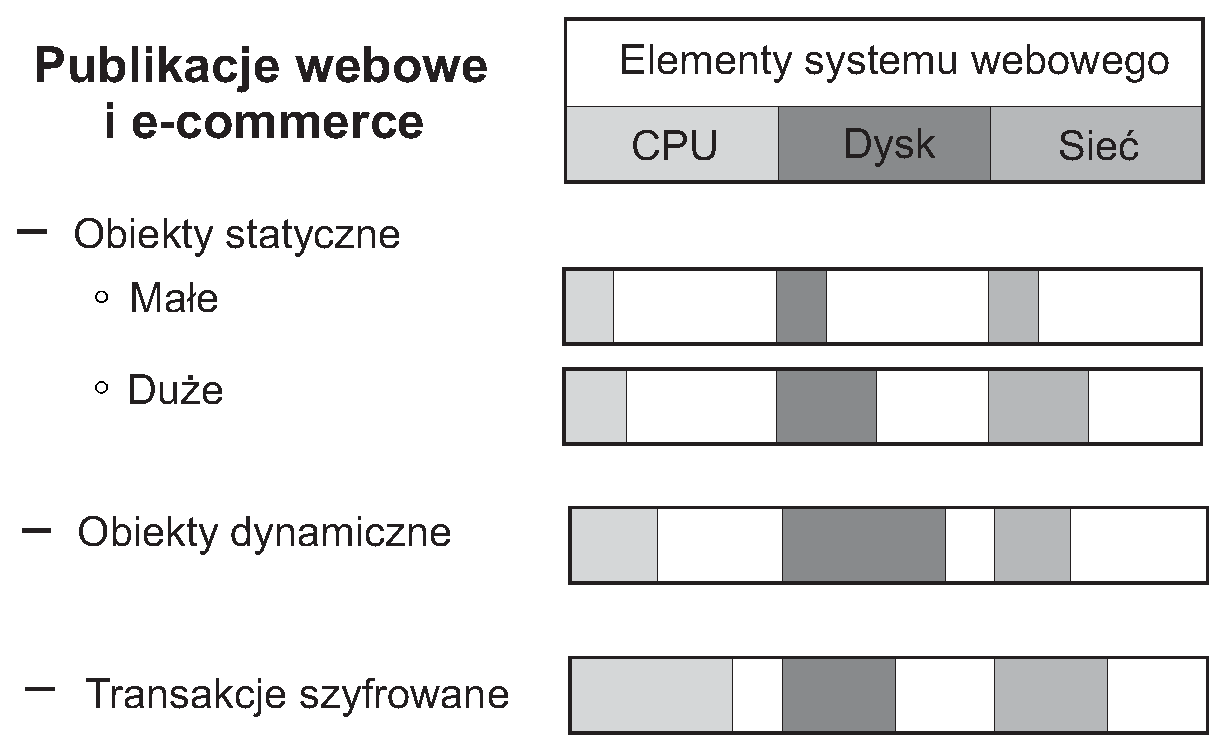
\includegraphics[width=3in]{./rysunki/charakterystyka_ruchu.eps}
\caption{Obciążenie poszczególnych elementów serwera WWW w zależności od typu połączenia.}
\label{charakterystyka}
\end{figure}

Prędzej czy później każdy administrator takiego serwera stanie przed problemem znalezienia sposobu na 
zwiększenie jego wydajności. Zwykle ze względu na specyfikę publikowanych informacji niewiele można zrobić ze 
średnim rozmiarem przesyłanego pliku. Podstawową metodą zwiększenia wydajności serwera jest zwiększenie 
przepustowości przyłącza. Sprzętowa modernizacja samego serwera nie przyniesie rezultatów w przypadku gdy 
,,wąskim gardłemi'' jest przyłącze. Jeśli jednak dysponujemy odpowiednio wydajnym przyłączem (np. linią ATM) 
,,wąskim gardłem'' jest na pewno serwer. 

Wydajność każdego komputera zwiększyć można dokupując większą ilość pamięci RAM i szybsze dyski twarde. 
W przypadku serwerów WWW jest to jednak rozwiązanie prowizoryczne. Lepsze efekty przynosi instalacja maszyny 
wieloprocesorowej. Niestety obecne implementacje TCP/IP nie wykorzystują wielowątkowości w stopniu, który 
umożliwiałby pełne wykorzystanie cech technologii wieloprocesorowej. Należy się spodziewać, że otwartych 
połączeń TCP będzie typowo więcej niż procesorów w serwerze. Gdyby obsługę stosu TCP/IP podzielić można było na 
niezależne wątki, których wykonanie przebiegać by mogło z podziałem czasu, to efektywność wieloprocesorowych 
serwerów WWW byłaby znacznie większa niż obecnie. Współcześnie stosowanie serwerów wieloprocesorowych nie 
przynosi korzyści tak dużych jak spodziewane. 
Dobrą metodą zwiększenia wydajności WWW jest stosowanie serwerów proxy, które na zasadzie pamięci cache 
przechowują część dokumentów serwisu i w ten sposób częściowo wyręczają serwer główny. 
Najbardziej efektywną i jednocześnie najbardziej zaawansowaną technologicznie metodą zwiększenia 
wydajności serwera WWW jest powielenie jego zawartości na jeden lub kilka dodatkowych serwerów i udostępnienie 
tej grupy pod jednym adresem IP. Rozwiązanie takie wymaga sprzętu lub oprogramowania, które z jednej strony 
ukrywałoby przed użytkownikami istnienie kilku serwerów o jednakowej zawartości a z drugiej dokonywałoby 
dystrybucji obciążenia pomiędzy te serwery w sposób maksymalizujący ich łączną wydajność.

\subsection{Serwery wielokomputerowe -- rozproszone}

\hspace{0.63cm}Żeby serwery WWW były wydajne oraz mogły pracować bez przerwy przez 365 dni w roku 24 godz. 
na dobę -- nie mogą pracować na jednym komputerze; wydajność, skalowalność a przede wszystkim odporność na 
awarie może zostać zrealizowana jedynie poprzez rozproszone serwery WWW, w których zapytania od klientów są
w odpowiedni sposób dystrybuowane do poszczególnych serwerów \cite{metodyalgorytmy}. 

Światowy trend w wykorzystywaniu na różne sposoby technologii World Wide Web jest coraz większy.
Znakomite darmowe serwery WWW (Apache, NCSA itp.), spora ilość przeglądarek internetowych
oraz olbrzymi rozwój internetu \cite{siecikomputerowe}, a także ogrone możliwości tej usługi spowodowały zwiększone 
zainteresowanie tą technologią.
Jednym z ostatnich niesłychanie modnych technologii internetowych wykorzystujących WWW jest handel 
elektroniczny skierowany tak do pojedynczego odbiorcy (\emph{Business to Customer-- B2C}) jak i współpracujących
firm (\emph{Business to Business}-- B2B). Poza tym również bardzo interesującym celem są serwery aplikacyjne.
Powoduje to jednakże konieczność utrzymania w sprawności serwisu przez cały rok -- bez 
przerwy. Nie oznacza to wyłącznie możliwości korzystania z tych serwerów, czyli bezawaryjnej pracy, ale również
uzyskanie jak najlepszego komfortu pracy z tymi systemami. Poza tym jeszcze jedną niesłychanie istotną rzeczą
przemawiającą za wielokomputerowymi serwerami WWW jest ich znakomita skalowalność (dużo tańsza od skalowalności
pojedynczych maszyn, które nie zawsze dadzą się rozbudowywać). Takich zalet nie posiada pojedyncza maszyna. Jej koszt zakupu, 
a także koszt rozbudowy -- przy zapewnieniu bezpieczeństwa i odporności na uszkodzenia jest olbrzymi. Fakt, że pojedynczą
maszyną łatwiej się administruje nie rekompensuje w pełni ułomności architektury von Neumanna. Wielokomputerowe serwery
(nie tylko WWW, ale także serwery obliczeniowe) mogą osiągać zawrotne wydajności, są praktycznie w nieskończoność skalowalne,
nadmiarowość tanich elementów (zamiast kupować trzy maszyny klasy mainframe -- można kupić sto komputerów klasy PC) decyduje
o ich odporności na uszkodzenia. Najlepszym przykładem jakości tej technologii jest najpotężniejsza z wyszukiwarek sieciowych --
GOOGLE\footnote{\emph{www.google.com}} pracująca na kilku tysiącach komputerow klasy PC, a zawierająca w swojej bazie informacje 
o ponad miliardzie trzystu milionach stron WWW (jest wykorzystywana przez większość serwisów webowych). Wadą
systemów klastrowych jest administracja i sposób współdzielenia obciążenia pomiędzy poszczególnymi nodami (istnieje jednakże
oprogramowanie darmowe umożliwiające równoważenie obciążenia serwerów WWW\footnote{\emph{www.linuxvirtualserver.org}}, a 
także serwerów obliczeniowych\footnote{\emph{www.mosix.org}}).

Trend ten nie znajduje odzwierciedlenia tylko w serwerach webowych. Konstrukcja wielokomputerowa pozwala na znacznie 
efektywniejsze zarządzanie zasobami i przydzieleniem zadań do zasobów. Pozwala także uzyskać ,,prawdziwe'' zrównoleglenie
obliczeń -- brak jest tu ,,kombinowanych'' metod uwspólniania zasobów i rozdziału żądań do magistral i pamięci obecnych
w typowych architekturach. Kolejną zaletą systemów nieneumanowskich jest możliwość zapewnienia bezpieczeństwa ciągłości
pracy w sposób dotąd niewykonalny. Przykładem spełnienia wszystkich tych cech są współczesne superkomputery i mainframy, 
z których doświadczeń korzystali współcześni twórcy nowoczesnych, skalowalnych technik webowych. Każdy superkomputer (SGI,
Hitachi, NEC, Intel, IBM) oraz system mainframowy (głównie IBM) składa się z szeregu (nawet kilkudziesięciu) nodów 
skonsolidowanych zwykle w jednej obudowie, a połączonych wysokoprzepustową siecią transmisyjną. Stąd wiele pomysłów zostało
zaczerpniętych i wykorzystanych przy tworzeniu rozposzonych architektur webowych.

Klasyczny system komputerowy obsługujący serwer webowy jest obsługiwany niskopoziomowo -- system operacyjny obsługujący
serwer webowy. W architekturze rozproszonego webu pomiędzy systemem operacyjnym poszczególnych nodów, a serwerem WWW (również
poszczególnych nodów) znajduje się logiczny układ koordynujący działania poszczególnych serwerów WWW tak aby działały jako
jeden rozproszony serwis. Ten system zarządzający odpowiada za: 
\begin{itemize}
\item rozdysponowywanie żądań przychodzących od klientów na poszczególne nody w taki sposób aby zapewnić zrównoważenie 
obciążenia poszczególnych maszyn, 
\item zapewnienie spójności danych na drodze klient--serwer www--klient, 
\item oraz sprawowanie kontroli nad poszczególnymi elementami klastra w ten sposób, aby zawsze, i odpowiednio szybko, było 
wiadomo, który komputer należy omijać ze względu na awarię.
\end{itemize}

Poniżej znajduje się opis i charakterystyka poszczególnych systemów równoważących obciążenia w rozproszonych serwerach 
webowych. 

\section{Przegląd skalowalnych systemów serwerów webowych}

Na rysunku \ref{proste_modele} przedstawiono wszystkie proste modele funkcjonalne systemów do równoważenia obciążeń w serwisach WWW. 
Ich charakterystyczną cechą jest to, iż w każdym wykorzystywany jest jeden mechanizm szeregowania. Można je traktować jak 
swego rodzaju klocki, z których budowane są rzeczywiste systemy. Cześć z nich odpowiada rzeczywistym systemom bez dodatkowych 
modyfikacji, część odzwierciedla rzeczywiste systemy dopiero we wzajemnych kombinacjach. Wyodrębnienie prostych modeli 
umożliwia zbudowanie przejrzystej taksonomii skalowalnych systemów serwerów webowych.

\begin{figure}[h]
\centering
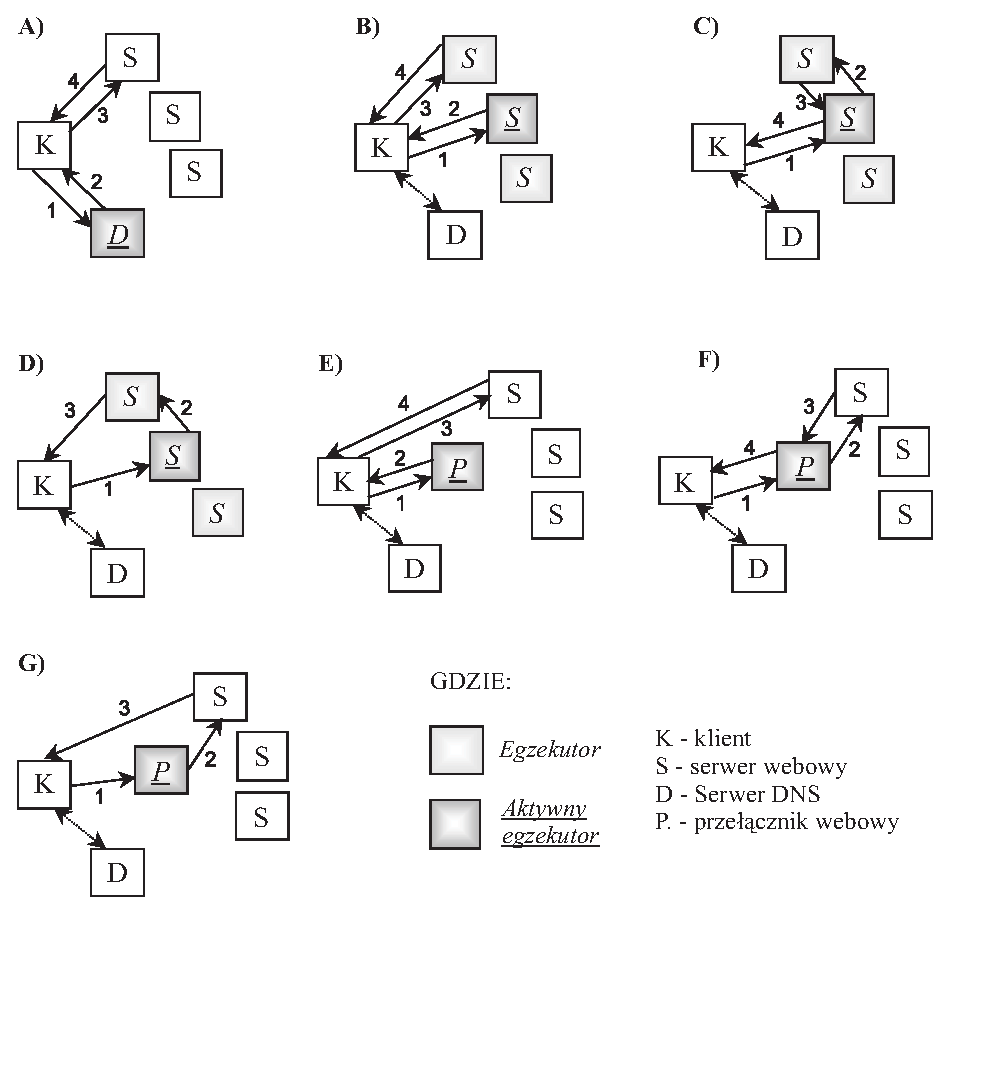
\includegraphics[width=4.9in]{./rysunki/modele_podstawowe.eps}
\caption{Podstawowe modele systemów do równoważenia obciążeń}
\label{proste_modele}
\end{figure}

\subsection{Podział ze względu na rozmieszczenie serwerów webowych}
Podział ten kształtuje się następująco:
\begin{itemize}
\item Klaster webowy. Jeśli serwery webowe są rozproszone lokalnie (skupione geograficznie), to mówi się o tzw. klastrze 
webowym (web--cluster). Z technicznego punktu widzenia klaster webowy funkcjonuje w obrębie sieci lokalnej. Każdy z prostych 
modeli przedstawionych na rys.\ref{proste_modele} może być implementowany w klastrze webowym. W przypadku modelu {\bf G}, ze względu na uwarunkowania 
techniczne transmisji żądań, może zajść potrzeba umiejscowienia klastra w obrębie podsieci sieci 
lokalnej \cite{modele15,modele20,LoadBalancingWithND}.
\item Rozproszone serwery webowe. Jeśli między rozproszonymi globalnie (rozproszonymi geograficznie) serwerami webowymi 
stosowany jest jakikolwiek mechanizm szeregowania, mówi się o rozproszonych serwerach webowych (distributed web--servers), w 
przeciwnym przypadku -- o lustrzanych serwerach webowych (mirror web--servers). Teoretycznie każdy model przedstawiony na rys.\ref{proste_modele}
może być implementowany wśród rozproszonych serwerów webowych, jednak ze względu na powstawanie dodatkowych opóźnień podczas 
transmisji zwrotnej w modelu {\bf F} oraz uwarunkowania techniczne transmisji żądań w modelu {\bf G}, oba wymienione modele mają 
zastosowanie głównie klastrach webowych.
\item Rozproszone klastry webowe. Szczególnym przypadkiem rozmieszczenia serwerów webowych jest kombinacja globalnego i 
lokalnego rozproszenia. Jeśli miedzy klastrami webowymi stosowany jest jakikolwiek mechanizm szeregowania, mówi się o 
rozproszonych klastrach webowych (distributed web--clusters). W przeciwnym przypadku -- o lustrzanych klastrach webowych (mirror 
web--clusters). Rozproszone klastry webowe można przedstawiać za pomocą kombinacji prostych modeli funkcjonalnych (rys.\ref{complex_modele} {\bf J, K}). 
\end{itemize}

\subsection{Podział i charakterystyka ze względu na umiejscowienie mechanizmu szeregowania}

Mechanizm szeregowania może być umiejscowiony: po stronie klienta, po stronie serwera, oraz jako osobny układu (serwer DNS,
dystrybutor).

\subsubsection{Podejście od strony klienta}

Główną zaletą stosowania mechanizmów rozpraszania obciążenia po stronie klienta jest całkowita niezależność od architektury 
serwera(ów), a przede wszystkim od miejsca ich rozmieszczenia (mogą być nie tyle geograficznie rozproszone, co wręcz 
nieskoordynowane jako całość). 

Rozwiązania w tym zakresie możemy podzielić na dwie podgrupy:
\begin{itemize}
\item mechanizmy równoważenia obciążenia implementowane w przeglądarkach i jako applety Java:
\begin{itemize}
\item w przeglądarkach poprzez API. Przeglądarka może aktywnie pełnić roleę w dystrybucji zapytań, pod warunkiem posiadania
informacji na temat adresów serwerów WWW. Wtedy, na podstawie zapytania otrzymanego od użytkownika, przeglądarka wybiera
serwer do przedłożenia zapytania. Klasycznym przykładem takiego rozwiązania jest mechanizm LB implementowany w przeglądarkach
firmy Netscape \cite{gliwice16,gliwice17}. Po wygenerowaniu zapytania przez użytkownika (tylko do serwera 
www.netscape.com), przeglądarka wybiera liczbę z zakresu od 1 do liczby znanych jej serwerów i kieruje zapytanie do węzła
o adresie www\emph{liczba}.netscape.com. Nie jest to rozwiązanie interesujące, gdyż liczba serwerów i adresów jest na stałe 
zakodowana w przeglądarce. Poza tym taki sposób rozdysponowywania ruchu (losowy) nie zapewnia równoważenia obciążenia pomiędzy
serwerami;
\item applety Java. O wiele ciekawszym od powyższego rozwiązaniem, jest implementacja specyficznych appletów Java. Gdy
użytkownik wysyła żądanie do serwisu, zamiast dokumentu HTML, pobiera applet Java. Applet ten zawiera adresy IP maszyn 
dostarczających ten serwis WWW \cite{gliwice18,gliwice19}. Applet może być modyfikowany przez program zbierający informacje o 
stanie serwerów (o ich obciążeniu) oraz o jakości połączenia sieciowego. Informacje te może wykorzystywać applet do
wyboru najbardziej odpowiedniego serwera do realizacji żądania. Główną wadą tego rozwiązanie jest generowanie 
dodatkowego ruchu w sieci (związanej z pobieraniem informacji o stanie obciążenia serwerów. Naturalnie jest ono również 
bezużyteczne gdy przeglądarka nie potrafi interpretować kodu Javy.
\end{itemize}
\item serwery Proxy. Jest to oparte na pomyśle po raz pierwszy wykorzystanym przez badaczy z Cambridge 
University \cite{gliwice20}. Mechanizm, który został zaimplementowany w serwer proxy, bazuje na informacji o 
osiągniętej wydajności podczas dotychczasowych transmisji. Klient otrzymuje listę zreplikowanych serwerów postrzeganych przez
użytkownika pod jednym adresem. Każdej pozycji na liście jest przypisana informacja o wydajności serwera. Za każdym razem, 
gdy klient utworzy połączenie z serwerem jest ona aktualizowana. Wybierany jest mirror na podstawie znajomości
najlepszej ze średnich wydajności serwera w ciągu ostatnich transmisji. Decyzja jest podejmowana z zastrzeżeniami: jeśli 
wydajność ostatniej transmisji spadła poniżej pewnego progu, serwer jest uważany za nieosiągalny. Wybór serwera proxy
wynikał z kilku ważnych powodów: ukrycie przed użytkownikiem faktu wyboru dokumentu między zreplikowanymi serwerami, brak
konieczności ingerencji w kod przeglądarki, oraz korzyść w postaci współdzielenia informacji o wydajności zreplikowanych 
serwerów między użytkownikami przeglądarek. Kilku klientów generuje większą liczbę zapytań, poprawiając w ten sposób wydajność
algorytmu równoważenia obciążenia \cite{gliwice20}. 
\end{itemize}

\subsubsection{Podejście od strony serwera}

Techniki równoważące obciążenie w oparciu o serwery wykorzystują dwupoziomowy mechanizm dystrybucji. Najpierw zapytania
klienta są przydzielane serwerom webowy w klastrze poprzez DNS. Następnie każdy serwer może przekazać otrzymane zapytanie
do innego serwera w klastrze. Rozwiązanie w oparciu o rozproszone szeregowanie pozwala wszystkim serwerom brać udział
w równoważeniu obciążenia w klastrze poprzez mechanizm przekazywania zapytań. Połączenie podejścia w oparciu o DNS oraz z
technikami przekierowywania zapytań poprzez serwery webowe prowadzi do rozwiązania większości problemów wynikających z polityki
szeregowania np.: niejednolita dystrybucja zapytań wewnątrz domeny, czy ograniczona kontrola nad zapytaniami.

Propozycje oparte na przekierowaniach serwerów różnią się w sposobie podejmowania decyzji. W następnym rozdziale są 
przedstawione dwie główne klasy rozwiązań: wykorzystujące funkcje redirekcji na poziomie protokołu HTTP oraz w oparciu o
mechanizm przepisywania pakietów. 

\subsubsection{Podejście od strony niezależnego węzła dystrybuującego zapytania}

W wyniku zapytania klienta o dane z serwera WWW -- w pierwszej kolejności następuje rozwinięcie nazwy domenowej serwera na
jego adres IP. Następnie adres IP może być reprezentowany przez wirtualny adres IP przypisany do klastra serwerów. Samo
rozwinięcie IP w adres serwera może być realizowane na różnych poziomach. Może to być przekierowanie do konkretnych zasobów na 
poziomie protokołu HTTP \cite{modele2} lub na poziomie protokołu IP oraz adresu URL przy zastosowaniu 
dystrybutora \cite{modele1,gliwice3}.

Na początku skupiano się na rozwiązaniach dotyczących podmiany nazwy serwisu na jego adres IP \cite{gliwice4}. Jednakże w 
związku z faktem ograniczeń takiego rozwiązania coraz większą uwagę poświęca się implementacji mechanizmów podmiany 
wirtualnego adresu IP na adres konkretnego hosta. Przykładami takiego podejścia są: Berkeley MagicRouter \cite{modele1}, 
CISCO Local Director \cite{gliwice13}, VirtualServer \cite{virtualserver} oraz IBM SecureWay Network Dispatcher \cite{GettingStarted}.

\begin{itemize}
\item Wykorzystanie serwera DNS -- 
egzekutorem jest serwer DNS lub inne urządzenie wspomagające albo przejmujące rolę serwera DNS. Należy uściślić, 
że chodzi tu o tzw. główny serwer DNS będący autorytatywnym źródłem informacji o określonej domenie (\emph{authoritative DNS}).
Jak opisano w Rozdziale 2 system DNS służy do odwzorowania symbolicznych nazw komputerów w Internecie na ich 
adresy IP. Funkcja ta, w niejako naturalny sposób, czyni serwer DNS dobrym miejscem na implementację mechanizmu 
równoważenia obciążeń. Pierwszą instalacją wykorzystującą  DNS do równoważenia obciążeń był serwis WWW NCSA 
(ang. \emph{National Center for Supercomputing Applications}). Zestawiono tam klaster dziewięciu serwerów WWW, który 
stanowił odrębny obszar DNS i był udostępniany pod nazwą www.ncsa.ninc.edu \cite{barylo28,barylo29}. Na podstawowym serwerze 
DNS  domeny (obszaru) ncsa.ninc.edu skonfigurowano oprogramowanie, które na zapytania o odwzorowanie nazwy 
www.ncsa.ninc.edu odpowiadało podając cyklicznie adresy kolejnych serwerów z klastera. Ten statyczny algorytm 
nazywany jest cyklicznym DNS lub RR--DNS (ang. \emph{Round--Robin DNS}). 

Podejście to jednak bardziej realizuje rozproszenie strumienia zapytań klientów niż równoważenie obciążenia serwerów WWW. W
rzeczywistości w Internecie jest wiele serwerów DNA i mają one układ hierarchiczny tzn. nie zawsze trzeba sprawdzać adres IP
w docelowym serwerze DNS. Oznacza to, że nie mamy wpływu na część zapytań, jakie są kierowane do serwera. W pewnym stopniu
poprawia sytuację zastosowanie sygnałów zwrotnych od serwera WWW do serwera DNS o przeciążeniu. Efekt jest odczuwalny dopiero 
po upływie czasu TTL (np. w momencie uszkodzenia maszyny i wyłączenia jej adresu z puli adresów serwera DNS). Aby efektywność
tego typu rozwiązań była jak największa, ważne jest prawidłowe oszacowanie tzw. ukrytego obciążenia, czyli wielkości zapytań
napływającego w czasie TTL. Do estymowania tej wielkości można zastosować funkcje heurystyczne \cite{gliwice4}.

\item Reverse proxy serwer

Typowe forward proxy (także transparent) zwykle używane przez prowajderów internetu przechowują strony najczęściej pobierane 
przez użytkowników. Z reverse proxy firmy mogą przechowywać specyficzną zawartość na 
serwerach podobnie jak prowajderzy i przekierowywać żądania (od klientów) do danych składowanych na tych serwerach poprzez 
proxy. Serwery 
proxy przechowują (keszują) informacje przychodzące od lokalnych serwerów. Zatem osiąganie stron jest o wiele szybsze -- jest 
pobierane (o ile istnieje) z keszu serwera proxy (stąd nazwa reverse -- ponieważ jego działanie jest dokładnie przeciwne do 
działania ,,zwykłego'' proxy serwera). 

Z technicznego punktu widzenia reverse proxy różni się od forward proxy jednym dodatkiem -- tym dodatkiem jest odpowiedni moduł 
tłumaczący adresy URL backendowych serwerów WWW tak jakby były to jego własne. Taki sposób działania ma jeszcze jedną ciekawą 
własność -- serwery backendowe mogą być specjalizowane, np. niektóre z nich mogą odpowiadać wyłącznie za przetwarzanie stron 
dynamicznych, inne statycznych, a jeszcze inne tylko stron zawierających sporo grafik. Wystarczy w module przeadresowań 
umieścić odpowiednią informację (tzn. jaki adres URL w sieci wewnętrznej ,,tłumaczyć'' na adres URL serwera proxy).

W związku z prostotą działania takiego systemu (znakomicie wykorzystywanego jako systemu zarządzającego wielokomputerową 
witryną WWW -- można równoważyć obciążenia, specjalizować serwery, oraz w dowolny sposób propagować ruch webowy) jest on często 
wykorzystywany. 

Oferta różnorakich produktów pełniących rolę reverse proxy serwerów jest bardzo bogata. Rozpościera się od produktów 
komercyjnych, takich jak Intel NetStructure, IBM Web Traffic Express (bedący elementem WebSphere Edge Server), po produkty 
niekomercyjne takie jak: Apache (najpopularniejszy serwer WWW -- może być również forward, transparent oraz reverse proxy 
serwerem, niestety na razie obsługuje jedynie protokół HTTP do wersji 1.0), oraz bardzo wydajne narzędzie: SQUID Web Proxy 
Cache\footnote{http://www.squid--cache.org} (obsługujący wszystkie wersje protokołu HTTP, mający też niezliczoną ilość funkcji 
dotyczących korzystania z tego systemu i bezpieczeństwa).

\item Wykorzystanie dystrybutora -- wyspecjalizowanego urządzenia.
Alternatywnym rozwiązaniem do DNS'a, pozwalającym na pełną kontrolę ilości zapytań nadchodzących do serwerów, jest 
zastosowanie dystrybutora. Rozszerza to wirtualizację adresu nie tylko na poziom URL, ale również na poziom protokołu IP. 
Dzięki temu można zastosować jeden wirtualny adres IP (single virtual IP address) IP--SVA dla klastra serwerów. Pozwala to na 
pełną kontrolę nad strumieniem zapytań kierowanych do serwerów.

Takie podejście ma jednak swoje wady. W systemie powstaje jeden węzeł obsługujący transmisję pakietów. W pewnych przypadkach 
wydajność całego systemu może zależeć od wydajności tego właśnie węzła. Wykorzystywane tutaj algorytmy są najprostsze, 
ponieważ dystrybutor obsługuje wszystkie nadchodzące pakiety i konieczne jest zminimalizowanie czasu poświęcanego na ich 
obsługę. Przykładem takiego rozwiązania jest SITA-V algorytm  \cite{gliwice10}.

Rozwiązania oparte na dystrybutorze ze względu na zastosowany mechanizm obsługi pakietów możemy podzielić na:
\begin{itemize}
\item metodę packet single--rewriting; rozwiązanie to polega na przekierowywaniu pakietów nadchodzących od klientów przez 
dystrybutor poprzez przepisanie docelowego adresu IP. Przykładem takiego rozwiązania jest mechanizm routera TCP opisany 
w  \cite{gliwice11}. Klaster serwerów WWW składa się z kilku węzłów oraz routera TCP, który pełni rolę dystrybutora.
Adres \emph{i} jest prywatnym adresem węzła, na którym uruchomiony jest serwer WWW. Wszystkie zapytania HTTP przychodzą do 
dystrybutora, ponieważ tylko IP--SVA jest adresem znanym publicznie (krok 1). Wybór serwera WWW dokonywany jest przez 
dystrybutor na podstawie algorytmu round--robin (krok 2). Przekierowanie pakietu do odpowiedniego serwera realizowane jest
dzięki przepisaniu adresu docelowego w pakiecie z IP--SVA na prywatny adres \emph{i} serwera w klastrze. Przepisywana jest 
również suma kontrolna w pakiecie, ponieważ zależy ona od adresu docelowego (krok 3). W związku z tym, że jedno żądanie składa 
się z kilku pakietów, dystrybutor przechowuje tablicę złożoną z par: adres źródłowy -- adres prywatny serwera WWW. Dzięki temu 
wszystkie pakiety pochodzące od jednego nadawcy mogą być kierowane do tego samego serwera WWW (krok 4). W następnym kroku 
serwer odsyła żądane dane do klienta (krok 6). Przed odesłaniem danych w pakiecie konieczne jest wpisanie w polu adresu 
nadawcy, adresu IP-SVA (krok 5).

Jakkolwiek rozwiązanie to jest przezroczyste dla klienta, to wymaga ono dużych zmian w kodzie routera oraz systemie 
operacyjnym serwera. Związane jest to z tym, że następuje podmiana adresów na poziomie TCP/IP. Z drugiej jednak strony 
rozwiązanie to jest bardzo odporne na uszkodzenia. W przypadku awarii serwera WWW jest on usuwany z tablicy routera i nie 
uwzględniany przy rozdziale pakietów aż do momentu naprawy. Architektura ta może być połączona z wykorzystaniem DNS'a. Pozwala 
to na skalowanie klastra nie tylko w sieci LAN, ale również sieci WAN.
\item metodę packet double--rewriting; architektura ta w swoim założeniu jest bardzo podobna do przedstawionej powyżej. 
Mechanizm polega na przepisywaniu adresów docelowych w pakietach nadchodzących od klientów. Dystrybutor następnie przesyła 
pakiety do odpowiedniego węzła obsługującego serwer WWW. W tym przypadku jednak wszystkie pakiety wracają z powrotem do 
dystrybutora. Mechanizm ten opiera się na architekturze NAT (Network Address Translation) opisanej w  \cite{modele17}.
W momencie odebrania nadchodzącego pakietu dystrybutor wybiera serwer WWW (krok 2), a następnie modyfikuje adres źródłowy oraz 
docelowy w nagłówku pakietu (krok 3). W drodze powrotnej pakietu dystrybutor ponownie zmienia adresy IP w nagłówku i przesyła 
dalej dane do klienta (krok 6). 

Znane są dwa rozwiązania oparte na tej architekturze. CISCO LocalDirector  \cite{gliwice13} oraz Magicrouter  \cite{modele1}
\item metodę packet forwarding by the dispatcher.
Packet forwarding jest podejściem odmiennym w stosunku do prezentowanych powyżej. Działanie jego polega na przesyłaniu 
pakietów do serwera w niezmienionej postaci zamiast przepisywaniu adresów w nagłówku. Podejście to pozwala na wykorzystanie 
tego samego rozwiązania w sieci LAN i WAN. Zarówno sama metoda jak i pakiet zostały opisane w dalszej części tej pracy.
\end{itemize}
\end{itemize}

\subsection{Podział ze względu na strategię rozmieszczenia mechanizmów szeregowania}
Z tej perspektywy rysuje się podział na dwie grupy modeli: z centralnym mechanizmem szeregowania i z rozproszonymi 
mechanizmami szeregowania.
\begin{itemize}
\item Centralny mechanizm szeregowania. Do tej grupy należą modele {\bf A, E, F, G} (rys.\ref{proste_modele}). W przypadku {\bf A} decyzja o przydzieleniu 
nazwie domenowej adresu IP najlepszego serwera webowego zapada centralnie, po stronie serwera DNS. Mimo scentralizowanego 
zarządzania, ze względu na specyfikę funkcjonowania DNS, skuteczność tego modelu jest 
niewielka \cite{modele14,ModeleFunkcjonalne}. W modelach  
decyzja o przekierowaniu żądania klienta zapada centralnie, w dedykowanym urządzeniu. W odróżnieniu od modelu, centralne 
zarządzanie oznacza stuprocentową kontrolę nad szeregowaniem.
\item Rozproszone mechanizmy szeregowania. W tej grupie decyzja o przekierowaniu żądania może zapaść na każdym serwerze, w 
którym zaimplementowano oprogramowanie egzekutora. Ideę rozproszonego szeregowania ukazują modele {\bf B, D, C} (rys.\ref{proste_modele}). Rozwiązanie takie zapobiega 
efektowi wąskiego gardła, na które w szczególności narażony jest model {\bf F}. Modele {\bf B} oraz {\bf D}
stosowane są głównie w celu poprawy skuteczności szeregowania w modelu {\bf A} (rys.\ref{complex_modele} {\bf H, I}).
\end{itemize}

\subsection{Podział ze względu na liczbę stopni szeregowania}
Systemy serwerów webowych mogą jednocześnie wykorzystywać jeden lub więcej mechanizmów szeregowania. Mówi się wówczas o 
skalowalnych systemach serwerów webowych z szeregowaniem jednostopniowym, dwustopniowym lub trójstopniowym. Nie spotyka się 
systemów o większej ilości stopni szeregowania. Modele systemów z szeregowaniem wielostopniowym można budować poprzez złożenie 
modeli prostych. Przykładowe modele złożone zostały przedstawione na rys.\ref{complex_modele}.

\begin{figure}[h]
\centering
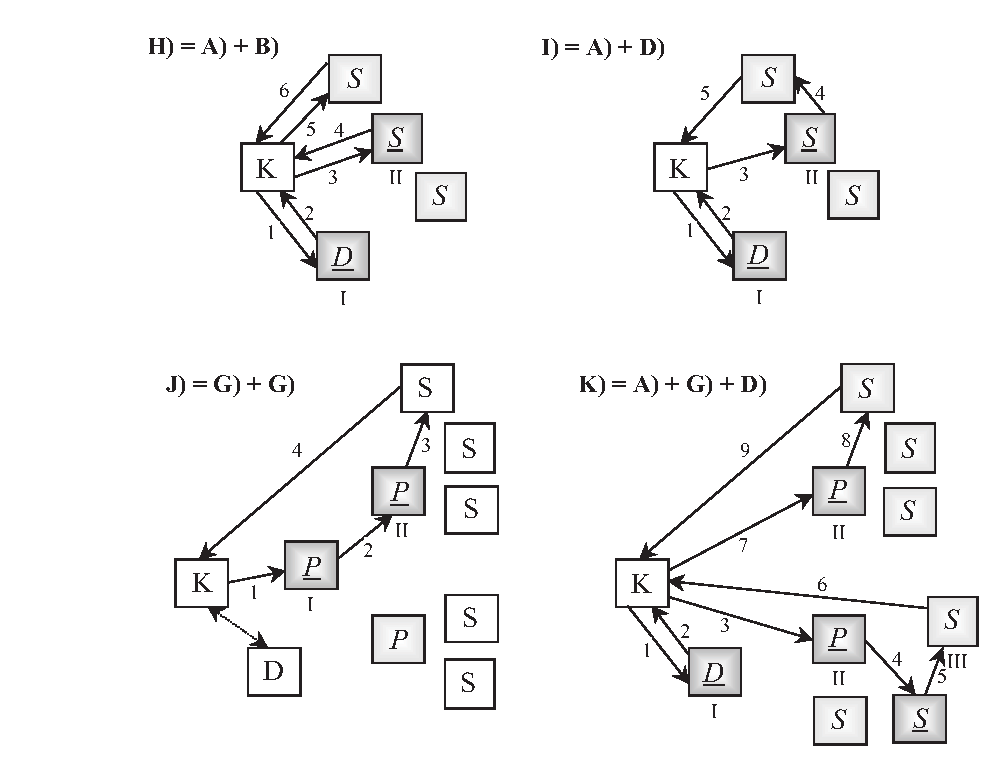
\includegraphics[width=4.9in]{./rysunki/complex_models.eps}
\caption{Złożone modele systemów do równoważenia obciążeń}
\label{complex_modele}
\end{figure}

\begin{itemize}
\item Systemy z szeregowaniem jednostopniowym. Systemy z szeregowaniem jednostopniowym odzwierciedlają modele: {\bf A, E, F, G} (rys.\ref{proste_modele}). 
W modelu {\bf A} egzekutor zintegrowany jest z serwerem DNS, natomiast w modelach{\bf E, F, G} rolę egzekutora pełni dystrybutor 
lub przełącznik webowy.
\item Systemy z szeregowaniem dwustopniowym. Przykładowe systemy z szeregowaniem dwustopniowym obrazują modele {\bf H, I, J} (rys.\ref{complex_modele}).
W przypadku {\bf H} oraz {\bf I} \cite{modele2,modele10,modele23,modele3} na pierwszym stopniu wykorzystywany jest model {\bf A}, natomiast na drugim, odpowiednio 
model {\bf B} lub {\bf D}. W obu przypadkach na pierwszym stopniu egzekutor zintegrowany jest serwerem DNS, natomiast na drugim rolę 
egzekutora pełni ten z serwerów webowych, który został wytypowany na poziomie serwera DNS. Przypadek {\bf J} ukazuje kaskadowe 
złożenie modeli {\bf G} (rys.\ref{complex_modele}) w celu szeregowania żądań w systemie rozproszonych klastrów webowych \cite{NDUsersGuide}. Na obu stopniach rolę egzekutora 
może pełnić dystrybutor lub przełącznik webowy. Model ten charakteryzuje się krótką drogą zapytań, jednak awaria pierwszego 
stopnia szeregowania unieruchamia cały system rozproszonych klastrów.
\item Systemy z szeregowaniem trójstopniowym. Przykład systemu z szeregowaniem trójstopniowym pokazuje model {\bf K} \cite{modele9}. Jest to 
system rozproszonych klastrów webowych, gdzie każdy z serwerów w klastrze ma wbudowany mechanizm szeregowania. Na pierwszym 
stopniu szeregowania wykorzystywany jest model {\bf A}, na drugim model {\bf G}, a na trzecim model {\bf B}, czyli na pierwszym stopniu 
egzekutor zintegrowany jest z serwerem DNS, na drugim role egzekutora pełni dystrybutor lub przełącznik webowy, natomiast na 
trzecim ten serwer webowy, który został wytypowany przez egzekutor na drugim stopniu. Każdorazowe zadziałanie trzeciego 
stopnia szeregowania, może powodować znaczne opóźnienia, jednak model ten jest bardzo odporny na przeciążenia i awarie. 
\end{itemize}

\subsection{Podział ze względu na poziom szczegółowości szeregowania}

\subsubsection{Szeregowanie na poziomie serii żądań o strony}
Aby zrealizować żądanie klienta o stronę umiejscowioną pod pewną nazwą domenową, mechanizm szeregowania, który jest 
zintegrowany z serwerem DNS, musi przydzielić tej nazwie adres IP najlepszego serwera webowego (hostname resolution). Ze 
względu na dużą bezwładność DNS kolejne żądania klienta o strony umiejscowione pod tą nazwą domenową będą przez pewien czas 
kierowane do tego samego serwera webowego. Przypadek, w którym szeregowanie żądań klientów odbywa się na poziomie serii żądań 
o strony, przedstawia model {\bf A}. 

\subsubsection{Szeregowanie na poziomie żądania o stronę}
W skład strony webowej wchodzi zwykle wiele obiektów. Na tym poziomie przekierowanie żądania o stronę pociąga za sobą 
przekierowanie serii żądań o jej elementy składowe. Mechanizm szeregowania wykorzystuje w tym celu właściwości protokołu HTTP 
(HTTP redirection \cite{modele18}). Przypadki, w których występuje tego typu szeregowanie, ukazuje model {\bf B} oraz {\bf E}. W przypadku modelu {\bf B}, gdy jeden 
z serwerów webowych otrzymuje od klienta żądanie o stronę, jeśli nie decyduje się sam zrealizować zlecenia, 
odsyła klientowi adres IP lub nazwę domenową lepszego od siebie serwera \cite{modele23}. W przypadku modelu {\bf E}, gdy przełącznik otrzymuje 
od klienta żądanie o stronę, odsyła mu adres IP lub nazwę domenową najlepszego serwera \cite{modele19}. 
Należy zaznaczyć, że może wystąpić tu zjawisko buforowania przez klienta adresu IP serwera, do którego nastąpiło 
przekierowanie. Można wówczas mówić o szeregowaniu na poziomie serii żądań o strony.

\subsubsection{Szeregowanie na poziomie żądania o obiekt}
Przypadki, w których szeregowanie odbywa się na poziomie żądania o obiekt, przedstawiają modele {\bf C, D, F} oraz {\bf G}. W tej grupie 
mechanizm szeregowania zajmuje się przekierowywaniem pakietów (packet redirection). Pakiety zawierające żądanie o obiekt muszą
w komplecie trafić do wybranego przez egzekutor serwera. Jednym ze sposobów realizujących ten cel jest zapisywanie wyników 
decyzji egzekutora w tzw. tablicy powiązań (binding table).
Ponieważ w modelu {\bf D} ruch pakietów powracających (znacznie 
większy niż w przypadku pakietów z żądaniami) jest kierowany do klienta z pominięciem serwera-egzekutora, model ten jest z 
powodzeniem implementowany. Charakterystyczną cechą modeli {\bf F, G} jest to, że egzekutor maskuje serwery webowe za pomocą 
jednego, wirtualnego adresu IP-SVA (single virtual IP address). Aby przekazać żądanie do konkretnego serwera, stosuje różne, 
niekiedy wyrafinowane techniki. Gdy egzekutor przekierowuje pakiety z żądaniami bez świadomości ich treści (content 
information blind), nazywany jest dystrybutorem (dispatcher, level 4 web-switch). Gdy egzekutor podczas podejmowania decyzji o 
przekierowaniu wykorzystuje informację zawartą w żądaniu (content information aware), nazywany jest przełącznikiem webowym 
(content switch, level 7 web-switch).
Należy podkreślić, że niniejszy podział dotyczy wariantu, gdzie w modelach {\bf F, G} rolę egzekutora pełni dystrybutor. 
W przypadku gdy egzekutorem jest przełącznik webowy, szeregowanie może odbywać się na poziomie żądania o obiekt, stronę oraz 
(dzięki umiejętności rozpoznawania znaczników cookie) serii żądań o strony.

\subsection{Podział ze względu na poziom kontroli zapytań}
Jest to podział wyodrębniający modele, w których egzekutory mają pełna kontrolę nad zapytaniami kierowanymi do systemu 
serwerów webowych.
\begin{itemize}
\item Pełna kontrola zapytań. Teoretycznie do tej grupy należą modele {\bf B, C, D, E, F} i {\bf G}. Klient, po otrzymaniu od 
serwera DNS adresu IP egzekutora, wszystkie zapytania kieruje tylko i wyłącznie do niego. W ten sposób egzekutor ma 
stuprocentową kontrolę nad zapytaniami. W rzeczywistości sytuacja taka zachodzi w przypadku modeli {\bf F} oraz {\bf G}. Warto zwrócić 
uwagę, że awaria lub zapchanie się egzekutora powoduje unieruchomienie całego systemu serwerów webowych. 
\item Częściowa kontrola zapytań. Typowym przypadkiem, w którym egzekutor sprawuje częściową kontrolę nad zapytaniami, jest 
model {\bf A}. Częściowa kontrola wynika ze specyfiki funkcjonowania systemu DNS. Również modele {\bf B, E} należy zaliczyć do tej 
grupy ze względu na możliwość występowania zjawiska buforowania przez klienta adresu IP serwera, do którego nastąpiło 
przekierowanie. Jeśli modele {\bf C} i {\bf D} byłyby implementowane samodzielnie, egzekutor, którego adres IP rozgłaszałby serwer 
DNS, sprawowałby pełną kontrole nad zapytaniami. Jednak w przypadku modelu {\bf D} typowym rozwiązaniem jest jego złożenie z 
modelem {\bf A} (model {\bf I} rys.\ref{complex_modele}). W takim przypadku każdy z egzekutorów implementowanych w serwerach webowych sprawuje częściową 
kontrolę nad zapytaniami kierowanymi do systemu serwerów webowych.
\end{itemize}

\subsection{Podział ze względu na poziom zaangażowania egzekutora} 
Egzekutor może być w różnym stopniu zaangażowany w przekierowywanie zapytań klienta. Może być również zaangażowany w proces 
przekazywania odpowiedzi. Rysują się tu cztery grupy modeli: bierne, zwrotne, jednokierunkowe oraz dwukierunkowe:
\begin{itemize}
\item Model bierny. Jest to model {\bf A}, w którym do egzekutora w ogóle nie trafiają żądania klienta o strony czy obiekty. 
Egzekutor odpowiada tylko na żądania o przełożenie nazwy domenowej na adres IP najlepszego serwera (klastra) webowego, nie 
biorąc bezpośredniego udziału w szeregowaniu zapytań klienta.
\item Modele zwrotne. Należą do nich modele {\bf B, E} (rys.\ref{proste_modele}). Egzekutor, po otrzymaniu żądania, zwraca klientowi adres IP lub nazwę 
domenową najlepszego serwera, aby ten mógł ponowić żądanie. W modelu {\bf B} może dodatkowo zapaść decyzja o obsłużeniu żądania 
przez bieżący serwer. Zaangażowanie egzekutora w proces przekierowywania jest w tym przypadku minimalne.
\item Modele jednokierunkowe. Należą do nich modele {\bf D} oraz {\bf G}\cite{modele15,modele20,NDUsersGuide}. Żądania, które osiągają egzekutor, przekierowywane 
są bezpośrednio do serwerów webowych. W modelu {\bf D} może dodatkowo zapaść decyzja o obsłużeniu żądania przez bieżący serwer. 
Dzięki odpowiednim zabiegom technicznym serwery kierują odpowiedzi bezpośrednio do klienta. Zaangażowanie egzekutora w proces 
przekierowywania jest w tym przypadku średnie.
\item Modele dwukierunkowe. Należą do nich modele {\bf C} i {\bf F} \cite{modele1,modele11,modele17} . Wszystkie żądania, które osiągają egzekutor, 
przekierowywane są bezpośrednio do serwerów webowych. W modelu {\bf D} może dodatkowo zapaść decyzja o obsłużeniu żądania przez 
bieżący serwer. Serwery webowe wszystkie odpowiedzi przesyłają do egzekutora, który musi je przekierowywać do klienta. 
\end{itemize}

\section{Witryny dynamiczne}

\hspace{0.63cm}Już nawet kilkudziesięcioma dokumentami World Wide Web, czyli bardzo niewielkim serwisem, trudno jest zarządzać, 
zmieniać i dodawać nowe fragmenty, czuwać nad poprawnością dostępnych w nim danych. Z drugiej jednak strony oprogramowanie 
stosowane do korzystania z World Wide Web jest bardzo proste, szeroko znane i szybko uaktualniane.

Większość informacji zapisanych na komputerach i wykorzystywanych w biznesie czy przez środki przekazu zgromadzona jest w 
bazach danych, w tym najcześciej w relacyjnych bazach danych. Bazy danych pozwalają na kontrolę nad danymi, analizowanie ich, 
ogranizację i prezentację użytkownikowi w jak najbardziej prosty i skuteczny sposób. Potrzebny jest jednak do nich dostep 
przez wyspecjalizowane oprogramowanie. W systemach klient/serwer jest to klient bazy danych; kolejny program, który musi 
poznawać użytkownik, program nie zawsze prezentujący najwyższy poziom możliwości technicznych czy łatwości komunikacji z 
użytkownikiem.

Oba te systemy, World Wide Web i bazy danych, stworzone są w tym samym celu -- efektywnego dostępu do informacji. Już po kilku 
latach rozwoju World Wide Web zorientowano się, że można je połączyć, biorąc z każdego, co najlepsze. Połączyć łatwość dostępu,
jaką niesie przeglądarka World Wide Web z wysokim stopniem organizacji oferowanym przez relacyjną bazę danych.

Sam serwer HTTP nie potrafi się jednak bezpośrednio porozumiewać z bazą; potrzebuje dodatkowego oprogramowania. Dawniej 
najlepszą metodą nawiązania kontaktu między serwerem HTTP a bazą było napisanie programu w standardzie CGI 
\footnote{ang. \emph{Common Gateway Interface}}. Program CGI przyjmuje informacje od serwera HTTP, przetwarza je i 
wysyła do bazy danych, baza 
danych wykonuje zlecane jej zadanie, wysyła efekt do programu CGI, który z kolei zwraca go przez serwer HTTP do klienta HTTP. 
Rezultatem jest najczęściej plik HTML. Dziś mechanizm porozumiewania się pozostaje taki sam, ale w miejsce programu CGI 
wchodzi program napisany w API serwera HTTP, na przykład ISAPI dla Microsoft Internet Information Server. To drugie 
rozwiązanie jest bardziej efektywne i pozwala na mniejsze obciążenie komputera, na którym działa serwer, niż w przypadku 
użycia programu CGI.

Można stworzyć serwis World Wide Web, który porozumiewa się z bazą danych. Można wpisywać do bazy nowe informacje, na przykład 
wypełniając ankietę marketingową, można przeglądać istniejące informacje, poprawiać je o ile mamy do tego prawo a także 
wyszukwiać potrzebne informacje.

Dokładnie takie same możliwości ma serwis wewnętrzny firmy -- intranetowy. Może on służyć do porozumiewania się z firmą 
oddziałów terenowych czy pracowników w podróżach służbowych, a także do zwykłej, codziennej komunikacji z bazą danych. 
Przeglądarka World Wide Web jest łatwiejszym w obsłudze i bardziej znanym użytkownikom oprogramowaniem niż specjalny klient 
bazy danych.

Do stworzenia takiego systemu potrzebny jest serwer HTTP i baza danych, a pomiędzy nimi program pośredniczący. Można napisać 
własne oprogramowanie pośredniczące, ale również skorzystać z gotowych produktów.

\section{Testowanie serwerów WWW}


Jak wiadomo słaba wydajność wprost przekłada się 
na niezadowolenia klientów, a niezadowolony klient opuści witrynę Web i
może nigdy już na nią nie wrócić \cite{savoia1,savoia2,savoia3}.

Przewidywanie jak witryna WWW będzie odpowiadać na specyficzne obciążenie
jest wielkim wyzwaniem. Od czasu jak sajty webowe stanowią kompleksowe
systemy zawierające elementy sprzętowe, programowe i sieciowe pochodzącymi od
różnych producentów, oraz posiadają bardzo różne profile wydajnościowe -- 
jest praktycznie niemożliwa predykcja, jak dany system zachowa się podczas
obciążenia. Jedynym pewnym sposobem sprawdzenia skalowalności systemu
jest przeprowadzenie testów wydajnościowych, w których natężenie i 
charakterystyka przewidywanego ruchu jest symulowana tak realistycznie jak
to jest możliwe. 

Testowanie obciążenia witryn webowych stanowi priorytet dla firm robiących interesy online. Jak wielu użytkowników z 
akceptowalnymi czasami odpowiedzi może obsłużyć strona ? Jest to niezwykle ważna informacja wykorzystywana do planowania 
kampanii reklamowych, estymacji budżetów branży IT a nawet do zwykłego dostarczania usług. I pomimo wagi tego problemu 
praktycznie większość testów obciążeniowych jest wykonywana niepoprawnie, ponieważ nie odpowiadają one rzeczywistym warunkom. 

Poniżej zostaną opisane elementy, niezbędne podczas konstrukcji
wysoce realistycznych i dokładnych testów wydajnościowych sajtów webowych (znajdują się również najczęściej popełniane w
typowych testach obciążeniowych błędy oraz sposób radzenia sobie z nimi):
\begin{enumerate}
\item Zrozumienie natury obciążenia

Pierwszym krokiem jest dokładne i obiektywne zrozumienie
natury obciążenia, jakie musi zostać wygenerowane, podczas symulacji ruchu na witrynie.

Niestety, testowanie obciążenia sajtów webowych jest dziedziną ralatywnie
nową (toteż słabo zrozumianą i udokumentowaną), a do tego jest bardzo ezoteryczną
dziedziną testów. Żeby odpowiednio zrozumieć naturę obciążeń należy możliwie
często korzystać z narzędzia dokonującego analizy logów naszego web serwera.
Daje to możliwość obserwacji detali odwiedzin każdego użytkownika: jego adresu IP, daty i czasu odwiedzin; jakie, 
ile i o jakiej wielkości dane pobierał, czy pobranie było zakończone sukcesem, czy nie oraz inne dane o sesji użytkownika, 
jego systemie operacyjnym i narzędziu z jakiego korzystał. 

    \begin{description}
    \item[Sesja użytkownika -- niezbędne informacje]\

Większość potrzebnych informacji jakie należy wyekstrahować podczas analizy logów są informacje związane z sesjami 
użytkowników\footnote{ang. \emph{user sessions}}. Testy obciążeniowe najbardziej związane są właśnie z sesjami użytkownika. 
Sesję użytkownika definiuje się jako sekwencję pobrań stron związaną z unikatowym (pojedynczym, identyfikowalnym) użytkownikiem.

Typowa witryna webowa jest wizytowana przez szeroką gamę użytkowników z szeroką gamą działań. Np. użytkownicy stron związanych 
z szeroko rozumianym e--commersem: niektórzy z nich przyszli pooglądać (\emph{browse}), niektórzy kupić, jeszcze inni 
sprawdzić status
zamówień. Nawet jeśli grupa klientów dokonuje pojedynczego działania, takiego jak kupowanie książki, każdy z tej grupy może to 
realizować na szereg sposobów. Niektórzy będą poruszać się ze strony na stronę bardzo szybko, raczej nie dbając o dokładne 
przeczytanie znajdujących się tam informacji, inni przeciwnie -- poruszają się powoli czytając każdą stronę bardzo uważnie. 
Niektórzy będą wyszukiwać czytając fragmenty wielu książek zanim zdecydują się na kupno jednej, inni skierują się od razu do 
miejsca zamówienia \emph{(purchase page)}.

Zrozumienie tej szerokiej gamy akcji, działań i zachowań jest niezbędne (krytyczne) dla zaprojektowania testów obciążeniowych, 
ponieważ dobrze zaprojektowany test powinien odzwierciedlać zachowania użytkowników tak precyzyjnie jak to tylko możliwe. 
Najlepszą metodą jest używanie analizatorów logów (podczas pracy witryny) oraz wydobycie kluczowej grupy zmiennych zachowania 
klientów najczęściej spotykanych na danym sajcie, adekwatnych do ruchu webowego. Niektóre ze zmiennych, na które zawsze 
powinno zwrócić się uwagę to:
	\begin{itemize}
	\item długość trwania sesji (mierzona w stronach);
	\item czas trwania sesji (duration) (mierzona w minutach i sekundach);
	\item typ stron wizytowanych podczas trwania sesji (strona domowa, strona informacji o produkcjie, strona informacji o kartach 
	kredytowych).
	\end{itemize}

Naturalnie nie są to wszystkie zmienne mające wpływ na charakterystykę obciążeniową sajtu -- oprócz nich należy wybrać jeszcze 
jakieś zmienne które o specyfice danej witryny decydują.

Taką specyfikę można zauważyć na przykładzie: siedmio--stronicowa sesja, której rezultatem jest zamówienie artykułu znacznie 
bardziej obciąża system niż siedmiostronicowa sesja, której wynikiem jest tylko przeglądanie dokumentów. Przeglądanie 
dokumentów jest zwykle związane z dokumentami statycznymi, zaś na sesję, której efektem jest dokonanie zakupu artykułu składa 
się cały szereg czynników takich jak: przeszukiwanie bazy danych zasobów witryny, użytkownika, transakcji kart kredytowych z 
weryfikacją (osobne systemy), a także wysłanie potwierdzającego zamówienie e--maila. Statystycznie rzecz biorąc pojedyncza 
sesja zakupu może pochłonąć zasoby sajtu tak jak dwadzieścia sesji statycznych \emph{(browsing)}. 

W podobny sposób można porównać zakupy dokonywane przez nowych i stałych klientów. Nowy użytkownik potrzebuje dokonać 
rejestracji, potwierdzenia i weryfikacji swoich danych, zaś stały już nie. Związane z bazą danych zakładanie użytkownika może 
być równe obciążeniu generowanemu przez pięciu stałych użytkowników, dlatego trzeba wyróżnić co najmniej dwa typy 
wykorzystania zasobów przy realizacji zakupów.

Gdy zostaną już zdeterminowane wszystkie zmienne związane z sesją użytkownika -- należy następnie znaleźć (zwykle również w 
logach) rangę i dystrybucję wartości tych zmiennych np. procentowa (w całości żądań) ilość żądanych stron podczas sesji.  Do 
takich celów można używać narzędzi statystycznych takich jak: odchylenie standardowe, jednakże najlepszym sposobem 
charakteryzowania większości zmiennych webowych testów obciążeniowych jest użycie rozproszenia jako wartości dyskretnej.

Wielkość detali i precyzję z jaką należy analizować te zmienne zależy od struktury sajtu (i jej komplikacji), czasu testów, 
oraz analizy wyników. 

    \item[Współbieżni użytkownicy]\

Zazwyczaj w testach obciążeniowych witryn webowych podaje się wartości obciążenia 
spowodowanego naraz współużytkującymi zasoby użytkownikami. Jednakże współbieżni użytkownicy nie powinni być widziani 
jako zmienna wejściowa w teście, ale jako rezultat wielu różnych czynników. A zwkle podaje się np. strona 
została przetestowana z obciążeniem 1000 współbieżnymi użytkownikami. Liczba współbieżnych użytkowników nie jest miernikiem 
obciążenia. Wartość ta jest rezultatem wydajności (zdolności do przyjęcia obciążenia) witryny. Efektem pracy na wolniejszym 
sajcie będzie większa liczba współbieżnych użytkowników. Można to pokazać na przykładzie -- jeśli na stronę loguje się trzech 
użytkowników w odstępnie czasowym 1min i pracują po 1 min (np. dokonują zakupów) -- to tylko i wyłącznie w zależności od 
wydajności witryny oraz jej obciążenia będzie 0, 2 i 3 naraz pracujących użytkowników. Zatem jeśli wydajność witryny webowej z 
jakiegoś powodu spada to wzrastać będzie liczba współbieżnych użytkowników. Trzeba jednakże dodać jeszcze jeden element -- 
jeśli wydajność sajtu spada (rośnie liczba współbieżnych użytkowników) rośnie także ilość użytkowników, którzy rezygnują z 
korzystania z jego zasobów. Jeśli witryna jest bardzo szybka to mogą się zdarzyć sytuacje, że ilość współbieżnych użytkowników 
będzie oscylować wokół zera (nawet przy ich dużej ilości). 

Z tych powodów używanie jako miernika obciążenia strony ilości współpracujących naraz użytkowników jest (jeśli ma być 
realistyczne) bardzo trudne, a wyniki zawsze odbiegają od rzeczywistych. Znacznie lepszym wskaźnikiem obciążenia witryny jest 
liczba sesji użytkownika wystartowana na godzinę. Ma to ważną zaletę -- jest to wartość stała, niezmienna w zależności od 
wydajności witryny w teście. Daje wskaźnik ilu użytkowników otrzyma stronę pierwszą witryny -- to czy ci użytkownicy ukończą 
swoją sesję, czy nie zależy już od zdolności strony do uniesienia danego obciążenia. I jest to właśnie ta wartość, którą się 
poszukuje podczas wykonywania testów.

    \item[Rezygnacja klientów]\

Kolejną ważną wielkością, niejednokrotnie źle szacowaną w testach, a mającą znaczny wpływ na testy obciążeniowe 
witryny jest rezygnacja klientów w trakcie sesji. Użytkownicy często rezygnują podczas sesji np. zakupów z powodu bardzo 
długich odpowiedzi serwera. Zmienną tą należy również brać pod uwagę podczas wykonywania testów obciążeniowych na 
przygotowywanym 
sajcie. Symulacja porzucania przez użytkowników sesji powinna być dokonana tak rzeczywiście jak to tylko możliwe. Jeśli nie, 
podczas testów będzie się symulować obciążenie tak wielkie jakie może nigdy nie nastąpić, lub wąskie gardła, które w 
rzeczywistości nigdy się nie pojawią. Pominie się zatem najbardziej istotne wyniki testów obciążeniowych: czyli 
użytkowników, którzy mogą porzucić sesję z powodu słabej wydajności. Zatem testy staną się nieużyteczne. W poniższej 
tabelce znajdują się przykładowe zależności pomiędzy liczbą opuszczających witrynę użytkowników, a czasem oczekiwania na 
określoną stronę.
\begin{table}[h]
\centering
\begin{scriptsize}
\begin{tt}
\begin{tabular}{|c|c|c|c|c|}
\hline
{Typ strony}&{\% opuszczających}&{\% opuszczających}&{\% opuszczających}&{\% opuszczających}\\
{}&{ 0--5 s }&{ 5--10 s }&{ 10--15 s }&{ 10--20 s }\\
\hline\hline
{Strona domowa}&{0\%}&{30\%}&{45\%}&{75\%}\\
\hline
{Stock quote}&{0\%}&{15\%}&{25\%}&{45\%}\\
\hline
{Stock Transaction}&{0\%}&{0\%}&{0\%}&{15\%}\\
\hline
{Account Information}&{0\%}&{5\%}&{15\%}&{35\%}\\
\hline
\end{tabular}
\end{tt}
\caption{Średni stopień porzucania witryny w \% dla różnych typów stron}
\label{porzucanie}
\end{scriptsize}
\end{table}
Jeśli zatem odpowiedź oczekiwania na stronę domową wynosi 5 sek. lub mniej nie obserwuje się ucieczki klientów. Jednakże 
powyżej tego czasu rezygnacja z oczekiwania staje się coraz wyraźniejsza, by w czasie 15--20 sek. $3/4$ obecnych na witrynie 
klientów już zrezygnowało. Jednakże należy zwrócić uwagę na jeszcze jeden związany z tym szczegół. Rezygnacja użytkowników 
zmniejsza obciążenie, zatem wydajność zaczyna się zwiększać, mniej użytkowników rezygnuje -- aż w końcu obciążenie z powrotem 
powoduje oczekiwania na realizację żądań o strony i cykl się powtarza. Jest to oczywiście przykład. Rezygnacja użytkowników z 
usług witryny jest bardzo ważną zmienną pokazującą, że dany sajt nie jest w stanie satysfakcjonująco zapewniać usług przy 
obciążeniu. Najczęściej oprogramowanie do testowania potrafi symulować rezygnację użytkowników, ale z ekstremalnych powodów -- 
zwykle 60--120sek. Jednakże takie wartości są nie do przyjęcia gdyż praktycznie nikt nie czeka tyle czasu. Aby móc wykonać 
testy obciążeniowe tak prawdopodobne jak to tylko możliwe, można skonfigurować testowaną witrynę w taki sposób, aby 
przekierowywać część użytkowników na wolniejszy mirror tej witryny. Można np. w ten sposób: 90\% ruchu jest kierowane na 
zwykły serwer, zaś 10\% na wolniejszy mirror, na którym np. strona domowa będzie serwowana później o 5 sek. W takiej 
konfiguracji należy ten dwuserwerowy system uruchomić na kilka godzin lub dni, do czasu otrzymania znaczących wyników. Po tym 
czasie należy dokonać analizy porzucających transakcje webowe klientów. Jeśli na zwykłym serwerze opuszczanie sesji po stronie 
domowej sięga 6\%, zaś na tym wolniejszym 20\%, trzeba się liczyć z opuszczaniem witryny przez 14\% klientów, którzy nie będą 
zbyt cierpliwi by poczekać kolejne 5 sek.

Porzucanie operacji webowych przez klientów nie jest interesującym wynikiem, samym w sobie -- daje pogląd na to jakie części 
sajtu są najbardziej obciążone w warunkach pracy. Jeśli np. strona domowa jest wyjątkowo wolna, większość użytkowników nawet 
nie rozpocznie sesji. Widać zatem, że odpowiednie symulowanie tego parametru jest bardzo istotne dla stworzenia wydajnego 
sajtu.

    \item[Dystrybucja zapytań o stronę]\

Kolejną ważną zmienną, której warto poświęć uwagę jest dystrybucja zapytań o  stronę. Ta ważna wartość określa o jakie strony 
są zapytania i w jakich proporcjach. Procedura zbierania tej danej jest dwustopniowa: najpierw należy zdefiniować 
skategoryzowane grupy stron, a następnie obliczyć udział procentowy żądań o strony w każdej grupie. 

    \end{description}

\item Estymacja wzrostu ruchu na witrynie

Kolejnym krokiem przy projektowaniu testów obciążeniowych jest zrozumienie pewnych kluczowych zmiennych -- niezbędnych do 
estymowania docelowego poziomu obciążenia:
    \begin{itemize}
    \item jak wzrasta całkowite obciążenie ruchu na sajcie;
    \item jaki jest poziom obciążenia pojedynczych pików, mających wpływ w całkowitym obciążeniu;
    \item jak szybko liczba użytkowników może wpłynąć na osiągnięcie maksimum piku obciążeniowego;
    \item jak długo trwają poszczególne piki.
    \end{itemize}

Przy pomiarze poziomu obciążenia można używać zmiennej: liczba sesji użytkowników na jednostkę czasu. Taki wybór wynika z jego 
prostoty w zrozumieniu i łatwości analizy.

    \begin{description}
    \item[Estymacja przyszłego ruchu webowego]\

Ocena szybkości wzrostu całkowitego obciążenia ruchu jest istotna, ponieważ rozmiar poziomu pików jest 
proporcjonalny do amplitudy całkowitego ruchu. Jeśli całkowity ruch wynosi np. 100000 sesji na tydzień, oznacza to piki o 
wielkości 1500 sesji na godzinę, zatem przy obciążeniu rzędu 200000 sesji na tydzień piki (chwilowe obciążenia) mogą sięgać 
3000 sesji na godzinę. 

Całkowity wzrost wielkości ruchu wynika z dwóch czynników: danych historycznych (o wzroście) oraz szacunków 
sprzedaży/marketingu. Aby estymować te wartości, należy dokonać analizy tygodniowego ruchu oraz dowiedzieć się od odpowiednich 
ludzi w firmie jak może się zmieniać ruch z miesiąca na miesiąc, oraz jak może wyglądać zainteresowanie na witrynie po 
specjalnych ofertach marketingowych. Z takich informacji można oszacować wartość obciążenia w czasie -- czyli przyszłe 
możliwości sajtu. 

    \item[Estymacja ruchu chwilowego]\

Po dokonaniu analizy wzrostu całkowitego obciążenia, należy estymować poziom natężenia ruchu chwilowego. Jest to niezbędne 
ponieważ ruch webowy jest raczej nierównomierny, a wiele sajtów doświadcza znaczących chwilowych obciążeń. Zwykle zdarza się 
to tylko kilka razy (raz, lub dwa w tygodniu lub kilka godzin dziennie). Gdy ruch webowy jest najwyższy. Przykładem są witryny 
pogodowe, na których nasilenie ruchu odbywa się w piątek i sobotę, ponieważ użytkownicy potrzebują danych pogodowych z powodu 
planów weekendowych. Natomiast (trading) handel sieciowy zwykle doświadcza największych obciążeń w okolicach czasu otwarcia i 
zamknięcia sklepu. 

    \item[Szacowanie przebiegu ruchu chwilowego]\

Estymowanie jak szybko osiągane jest docelowe chwilowe obciążenie, oraz przez jak długi czas jest utrzymywane jest tak ważne 
jak estymacja amplitudy chwilowych obciążeń. Można to pokazać na przykładach:

Sprzedaż online (stock) doświadcza zwykle ekstremalnie ostrych chwilowych natężeń ruchu (pików) w różnym czasie jak np. 
otwarcie sklepu. W ciągu kilku minut witryna przechodzi od nie przyjmowania zgłoszeń po przyjmowanie ich tysięcy naraz. Test 
obciążeniowy powinien dla tego typu sajtów generować tak specyficzne wysokie chwilowe obciążenia zwykle w czasie od pięciu do 
dziesięciu minut. 

Sprzedaż ubrań online, może doświadczać innej charakterystyki obciążeniowej. Tutaj testy obciążeniowe powinny generować wzrost 
obciążenia (do docelowego maksymalnego) w czasie rzędu jedna dwie godziny. Szybszy wzrost może odbiegać od sytuacji 
rzeczywistej. 

Czas trwania pików obciążeniowych jest również bardzo ważny -- witryna radząca sobie z wysokim obciążeniem trwającym pięć do 
dziesięciu minut może się zupełnie załamać podczas dłużej trwającego wysokiego ruchu. 
    \end{description}

\item Dokumentowanie i projekt

Gdy wszystkie powyżej wymienione informacje zostaną zebrane można zaprojektować odpowiedni do danych warunków test 
obciążeniowy.

Kluczowymi elementami takiego testu są:
    \begin{itemize}
    \item cele testu: zdeterminowanie jakiemu obciążeniu oraz w jaki sposób będzie poddawana witryna, a także czy wraz z 
    wzrastającym ruchem jest w stanie mu podołać;
    \item kryteria jakie będą spełnione podczas trwania klienckiego żądania -- tzn. np. maksymalny czas oczekiwania na stronę lub 
    nawet czas po jakim żądanie może zostać odrzucone;
    \item opis skryptów testowych i ich typy: np. scrypt opisujący trójstronicowe żądanie (strona domowa >> informacja o produkcie 
    >> zamowienie) oraz procentowe wykorzystanie tych typów skryptów;
    \item opis scenariusza czyli użycie skryptów testowych, czas ich uruchamiania oraz ich udział procentowy w całości testu, a 
    także czas i szybkość narastania obciążenia (piki obciążeniowe).
    \end{itemize}
\end{enumerate}
